\documentclass{article}
\usepackage[T1]{fontenc}
\usepackage{lmodern}
\usepackage{graphicx}
\usepackage{amsmath,amssymb}
\usepackage[a4paper,margin=2cm]{geometry}
\usepackage[absolute,overlay]{textpos}
\setlength{\TPHorizModule}{1mm}
\setlength{\TPVertModule}{1mm}
\usepackage[indonesian]{babel}
\usepackage{hyperref}
\setlength{\emergencystretch}{2em}
% unit: Halaman 41

\begin{document}

% === Halaman 41 (llm) ===

\section*{InvShiftRows()}

\begin{itemize}
    \item \textit{InvShiftRows} sama seperti \textit{ShiftRows} namun melakukan pergeseran dalam arah berlawanan (ke kanan) untuk tiap-tiap baris pada tiga baris terakhir di dalam \textit{state}
\end{itemize}

\vspace{10mm}

% deskripsi: Diagram ilustrasi proses InvShiftRows yang menunjukkan transformasi matriks state dari bentuk awal ke bentuk setelah pergeseran kanan pada baris kedua, ketiga, dan keempat.
% bbox normalisasi: [0.1300, 0.5000, 0.8500, 0.7500]
\begin{textblock*}{151.20mm}(27.30mm,148.50mm)
\noindent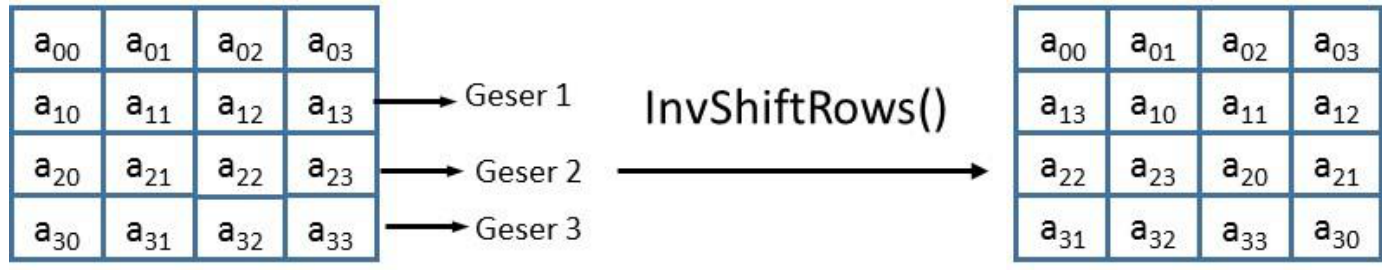
\includegraphics[width=151.20mm,height=74.25mm]{../../images/llm/page_041_img_01.png}%
\end{textblock*}

\end{document}
